\section{Task 4: Less or More?}
\label{sec:task4}

\subsection{Results for 50 L and 25000 L}
\label{sec:task4-results}
The amber-beer optimisation is repeated for 50 L, 5000 L, and 25000 L. The relaxation, rounded-process solution, and MILP solution coincide for these three cases because the relaxed process variables are already integral.

\begin{table*}[!t]
\renewcommand{\arraystretch}{1.15}
\caption{Task 4 Volume Comparison}
\label{tab:task34-volume-comparison}
\centering
\small
\begin{tabular}{@{}rrrrr@{}}
\toprule
Beer volume (L) & Relaxation cost & Rounded cost & MILP cost & MILP cost per litre \\
\midrule
50 & 67.767 & 67.767 & 67.767 & 1.355 \\
5000 & 4497.687 & 4497.687 & 4497.687 & 0.900 \\
25000 & 13420.213 & 13420.213 & 13420.213 & 0.537 \\
\bottomrule
\end{tabular}
\end{table*}

\subsection{Marked Costs on Task 1 Plot}
\label{sec:task4-marked-plot}
The three production volumes from Table~\ref{tab:task34-volume-comparison} are marked on the cost-volume plot from Task 1.

\begin{figure}[!t]
\centering
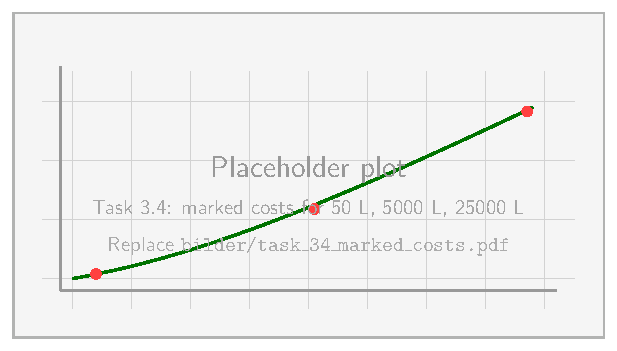
\includegraphics[width=\linewidth]{bilder/task_34_marked_costs}
\caption{Task 4 costs marked on the Task 1 cost-volume plot. Replace this placeholder with the plot exported from \texttt{task\_34.ipynb}.}
\label{fig:task34-marked-costs}
\end{figure}

\subsection{Cost per Litre Discussion}
\label{sec:task4-discussion}
The cost per litre decreases as the production volume increases. The 50 L batch is expensive per litre because any fixed process cost is spread over very few litres. Larger batches spread fixed costs over more output, so the cost per litre is lower. The 25000 L case has the lowest cost per litre in Table~\ref{tab:task34-volume-comparison}.

% Values and Figure \ref{fig:task34-marked-costs} come from task_34.ipynb.
